\documentclass[12pt, letterpaper]{article}
\usepackage[utf8]{inputenc}
 \usepackage[letterpaper, margin=1in]{geometry}
 \usepackage{amssymb}
\usepackage{amsmath}
 \usepackage{enumitem}
\usepackage {listings}
\usepackage{pgfplots}
\usepgfplotslibrary{external}
\usepackage{graphicx}

\title{CS425 Project1 (Report)\\Multiple Linear Regression Analysis}
\author{Ksenia Burova}
\date{October \(1^{st}\), 2017}

\begin{document}
\maketitle

\noindent {\bf Abstract:} In machine learning, multiple regression is a function of multiple inputs (discrete or numeric), that has one output that is a class code or continuous value. \\
In this project, the goal was to predict the gas milage of automobiles from their other multiple attributes by using multiple linear regression. We were given two files, one with data and another one with attribute information for that data. Six values for horsepower were missing, and had to be skipped or predicted. Data attributes contained both, discrete and numeric values. We had to compare performance of data with and without standardization. After calculating weights, we had to analyze which attribute was the best in predicting gas milage. 

\begin{enumerate}[label=\Roman*.]
	
	{\bf \item Project data} \\
	
	The following attributes are provided:
	\begin{itemize}
		\item    mpg:           continuous  -  {\bf to be predicted}
		\item    cylinders:     multi-valued discrete
		\item    displacement:  continuous
		\item    horsepower:    continuous
		\item    weight:        continuous
		\item    acceleration:  continuous
		\item    model year:    multi-valued discrete
		\item    origin:        multi-valued discrete
		\item    car name:      string (unique for each instance) - {\bf not used}
	\end{itemize}
	
	We represent data ( all but milage and names) in a matrix form:\\
	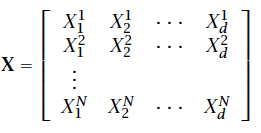
\includegraphics[scale=0.5]{pics/matrix.png} \\
	
	Each column is a single attribute, each row is a single experiment or data sample (in our case, all params for one unique car).
	
	{\bf \item Resolving missing values} \\
	
	There are six observations where horsepower attribute is not defined. Sometimes it is the best strategy to discard those observations. Another way is  to estimate those values using {\it imputation} method. There is mean imputation and imputation by regression possible. \\
	I've used two approaches: ignored observations with missing values and I tried mean imputation. 
	
	{\bf \item Calculating weights with Multiple Regression} \\
	(Equations are copied from the textbook) \\
	
	Going back to multiple regression, our numeric output is vector {\it r} which represents milage attribute.  We have a weighted sum of attributes \( x_1, x_2 ... x_d\) and some noise.  \\
	Here is a multivariate linear model: \\
	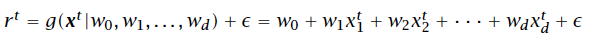
\includegraphics[scale=0.5]{pics/model.png} \\
	We may assume error to be normal with mean 0 and constant variance. To maximize the likelihood we will minimize the sum of squared errors: \\
	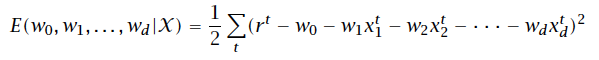
\includegraphics[scale=0.5]{pics/errors.png} \\
	Taking derivative with respect to parameters we get the normal equations: \\
	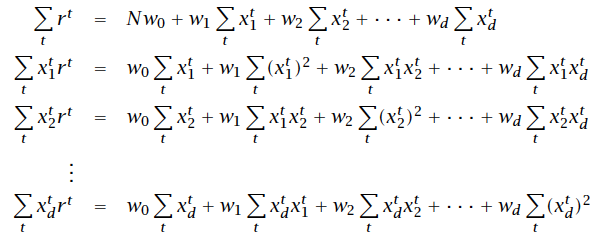
\includegraphics[scale=0.5]{pics/normal.png} \\
	We now can define the matrix of attributes (as before) but with first column being all ones, since in our model \(w_0\) term is the same as \(w_0 \cdot 1 \). We can define a vector of all weights, and an output vector which is our milage values. So we get: \\
	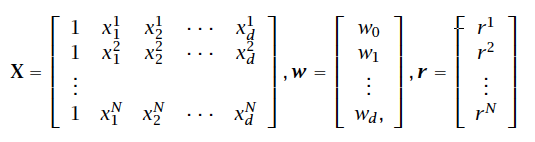
\includegraphics[scale=0.5]{pics/attr.png} \\ 
	Then the normal equations can be written this way now: \\
	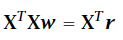
\includegraphics[scale=0.5]{pics/eq.png} \\
	And we can derive weights: \\
	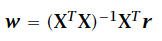
\includegraphics[scale=0.5]{pics/weights.png} \\
	So the goal is to compute and analyze these weights.
	
	{\bf \item Program structure} \\\\
	I've written my application in Python as was suggested. I've used {\it numpy} library to use matrix operations on vectors. \\
	I have two files.  I've defined a class {\it MultRegression} in one and have written functions for calculating mean, standard deviation, data standardization and weights. My second one is basically like main, I create an instance of the class and pass parameters.\\
	I pass 3 parameters to my class (I manually modify them in main function): 
	\begin{enumerate}[label=\arabic*.]
		\item Data file name 'auto-mpg.data'
		\item Boolean value to decide if i need to standardize my data. 1 - yes, 0 - no
		\item Boolean value to decide if I need to skip data with missing attributes. 1 - yes, 0 - no
	\end{enumerate}
	I've tested my functions on smaller data examples and matrices before running it on givven data.
	
	{\bf \item Expectations} \\
	
	Before running my experiment I decided to look at all the given attributes to figure out what effect on gas milage those can possibly have. These were my expectations:
	\begin{itemize}
		{\bf \item Cylinders + Displacement} \\
		Displacement is how much air engine consumes, and more air it consumes more gas get consumed as well. Displacement pretty much depends on number of cylinders in a car, as we see:\\  
		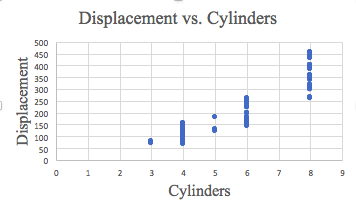
\includegraphics[scale=0.7]{pics/1.png} \\
		So, with both of these parameters increasing, out gas milage should be decreased.
		
		{\bf \item Weight + Horsepower} \\
		Weight of the car means a lot too. Heavier the car then harder that motor has to work.So I would expect this parameter to have the most negative effect on milage. Also, to increase the ability of motor to handle more work we have to increase its horsepower parameter. So greater weight would probably cause in bigger horsepower for that car. \\
		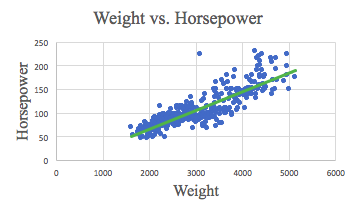
\includegraphics[scale=0.7]{pics/2.png} \\
		So If car has a bigger weight and the engine has to do more work then heavier cars should have lower milage. But is it when car doesn't have enough horsepowers? Will have to see. I think it depends. I think if horsepower attribute is hight enough for car's weight , weight affect should be fine. But now, greater horsepower might involve something else in engine construction that would probable eat up a bit more gas.
		
		{\bf \item Acceleration} \\
		I think higher acceleration should cause in lower milage, can't really explain why as I'm not a car  specialist. Intuitively,  when we speed up engine has to work harder to move the car forward faster. We have to apply some power that we have to get from gas.\\
		
		{\bf \item Model Year + Origin} \\
		I really don't know what to expect from these two attributes. I would assume that newer cars have better  transmissions and thus more efficient gas usage. Something similar may be going on with origin. \\
		Overall, I expect all parameters to have some effect on gas milage in a negative way. And all of these may depend on each other overall. 
		
	\end{itemize}
	
	{\bf \item Results} \\
	
	The first time I ran my program I skipped lines with missing attributes and I didn't standardize parameters. I received following values for weights:
	\begin{verbatim}
	[ -1.80586717e+01  -4.18254893e-01   1.88870416e-02  -1.13851962e-02
  	-6.71865820e-03    1.02620868e-01   7.56755050e-01   1.41751561e+00]
	\end{verbatim}
	It is really hard to analyze these values since they are so little, it's hard to say if value is close to 0 or not and that's the case when attribute has almost no affect on dependent variable. Also different data types and ranges my cause in sign switch for coefficients. So, usually data standardization is needed when we use attributes of different types that have different value ranges. Here are results after standardization:
	\begin{verbatim}
	[ 23.45731655  -0.71059527   1.96696134  -0.43435854  
	 -5.68269173  0.28265403   2.79477515   1.135508]
	\end{verbatim}
	
	Seems like Cylinders and Horsepower have some negative effect on gas milage, and weight has the biggest one, as expected. Other parameters seem to have positive effect, which I expected only for year and origin. Acceleration value is very small any way, I wonder if it has something to do with other parameters for it to be positive. Or maybe I didn't understand its meaning correctly.  Displacement also was expected to have negative effect but here displacement depends on cylinders very much and may be it has something to do with that. The order in which attributes have the most affect is the following:\\
	
	{\bf Acceleration, Horsepower, Cylinders, Origin, Displacement, Year , Weight. }\\
	
	So, weight of the car is probably a key factor in calculating gas milage which makes sense, the workflow of other car parts may depend on energy that engine has to produce. Same with year, newer cars are expected to be more efficient in gas usage.\\
	
	Now, I estimated horsepower for samples with missing values and added those:
	\begin{verbatim}
	[ 23.44591837  -0.84051891   2.07930256  -0.65163644  
	-5.49205044   0.22201407   2.76211888   1.14731588]
	\end{verbatim}
	
	Values didn't change much in sign. Attributes effect negativity is still the same. The absolute values for some attributes have changed. Horsepower has a little more affect on milage. But there is no garantee
	that we estimated those missing values correctly, so probably this result has more noise than previous.
		
	Now let's draw a plot of milage(weight, year) for given data: \\
	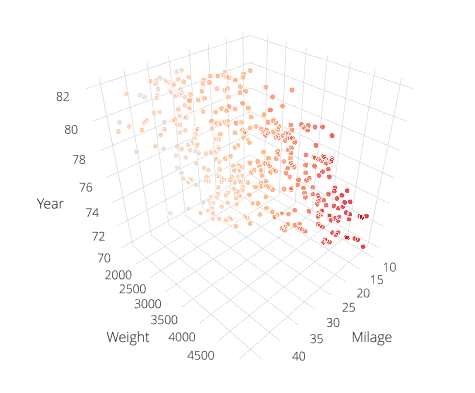
\includegraphics[scale=0.8]{pics/4.png} \\
	
	The color shift to red shows, how increasing car weight decrease milage, at the same time if look at year and milage, milage is higher for a bigger year.
	
\end{enumerate}
	
\end{document} 